\documentclass[xetex,mathserif,serif,aspectratio=169]{beamer}

\usepackage{xltxtra}
\usepackage{color}
\usepackage{url}
\usepackage{listings}
\usepackage{fontspec}
\usepackage{geometry}
\usepackage{lastpage}
\usepackage{fancyhdr}
\usepackage{amsmath}
\usepackage{amsthm}
\usepackage{amssymb}
\usepackage{blkarray}
\usepackage{multicol}
\usepackage{relsize}
\usepackage{listings}
\usepackage{xunicode}
\usepackage{xltxtra}
\usepackage{color}
\usepackage{url}
\usefonttheme[onlymath]{serif}

\definecolor{solarized@base03}{HTML}{002B36}
\definecolor{solarized@base02}{HTML}{073642}
\definecolor{solarized@base01}{HTML}{586e75}
\definecolor{solarized@base00}{HTML}{657b83}
\definecolor{solarized@base0}{HTML}{839496}
\definecolor{solarized@base1}{HTML}{93a1a1}
\definecolor{solarized@base2}{HTML}{EEE8D5}
\definecolor{solarized@base3}{HTML}{FDF6E3}
\definecolor{solarized@yellow}{HTML}{B58900}
\definecolor{solarized@orange}{HTML}{CB4B16}
\definecolor{solarized@red}{HTML}{DC322F}
\definecolor{solarized@magenta}{HTML}{D33682}
\definecolor{solarized@violet}{HTML}{6C71C4}
\definecolor{solarized@blue}{HTML}{268BD2}
\definecolor{solarized@cyan}{HTML}{2AA198}
\definecolor{solarized@green}{HTML}{859900}
\definecolor{yaleblue}{HTML}{0E4C92}

\newcommand{\yellow}[1]{\textcolor{solarized@yellow}{#1}}
\newcommand{\orange}[1]{\textcolor{solarized@orange}{#1}}
\newcommand{\red}[1]{\textcolor{solarized@red}{#1}}
\newcommand{\magenta}[1]{\textcolor{solarized@magenta}{#1}}
\newcommand{\violet}[1]{\textcolor{solarized@violet}{#1}}
\newcommand{\blue}[1]{\textcolor{solarized@blue}{#1}}
\newcommand{\cyan}[1]{\textcolor{solarized@cyan}{#1}}
\newcommand{\green}[1]{\textcolor{solarized@green}{#1}}
\newcommand{\yblue}[1]{\textcolor{yaleblue}{#1}}
\newcommand{\base}[1]{\textcolor{solarized@base01}{#1}}


\defaultfontfeatures{Mapping=tex-text}
\hypersetup{pdfstartview={FitH}}

\newcommand{\old}[1]{\fontspec[Alternate=1,Ligatures={Common}]{Hoefler Text}\fontsize{18pt}{30pt}\selectfont #1}%
\newcommand{\oldA}[1]{\fontspec[Alternate=1,Ligatures={Common, Rare}]{Hoefler Text}\fontsize{12pt}{15pt}\selectfont #1}%
\newcommand{\oldB}[1]{\fontspec[Ligatures={Common}]{Didot}\fontsize{12pt}{15pt}\color{solarized@base02}\selectfont #1}%
\newcommand{\tfont}[1]{\fontspec[Alternate=1,Ligatures={Common}]{Hoefler Text}\fontsize{12pt}{20pt}\selectfont #1}%
\newcommand{\dfont}[1]{\fontspec[Ligatures={Common}]{Didot}\fontsize{12pt}{12pt}\selectfont #1}%

\setbeamerfont{title}{family=\old}
\setbeamerfont{author}{family=\tfont}%
\setbeamerfont{frametitle}{family=\oldA}
\setbeamerfont{date}{family=\dfont}

\setbeamertemplate{navigation symbols}{}
\setbeamertemplate{footline}[text line]{%
  \parbox{0.99\linewidth}{
    \normalsize\vspace*{-24pt}\hfill{\color{solarized@base00}\insertframenumber/\inserttotalframenumber}
  }
}


\setlength{\parindent}{0pt}
\setlength{\parskip}{12pt}

\setbeamercolor{structure}{bg=solarized@base3, fg=solarized@base02}
\setbeamercolor{titlelike}{fg=solarized@cyan}
\setbeamercolor{title}{fg=solarized@blue}
\setbeamercolor{subtitle}{fg=solarized@magenta}
\setbeamercolor{alerted text}{fg=orange}
\setbeamercolor{itemize}{fg=solarized@base02}
\setbeamercolor{background canvas}{bg=solarized@base3}
\setbeamercolor{enumerate subitem}{fg=solarized@base02}

\newcommand{\minimize}{\mathop{\mathrm{minimize}}}
\newcommand{\argmin}{\mathop{\mathrm{arg\,min}}}
\newcommand{\argmax}{\mathop{\mathrm{arg\,max}}}
\newcommand{\st}{\mathop{\mathrm{subject\,\,to}}}


\usepackage[]{algorithm2e}
\usepackage{../kbordermatrix}

\begin{document}

%%%%%%%%%%%%%%%%%%%%%%%%%%%%%%%%%%%%%%%%%%%%%%%%%%%
\begin{frame}[fragile] \frametitle{} \oldB \small

\vfill

{\fontsize{0.7cm}{0cm}\selectfont Lecture 19 \\\vspace{0.2cm}
Word Vector Embeddings}\\\vspace{0.5cm}
18 April 2016

\vspace{2cm}

\begin{minipage}{0.6\textwidth}
Taylor B. Arnold \\
Yale Statistics \\
STAT 365/665
\end{minipage}
\hfill
\begin{minipage}{0.3\textwidth}\raggedleft

\includegraphics[scale=0.3]{../yale-logo.png}
\end{minipage}%

\end{frame}

%%%%%%%%%%%%%%%%%%%%%%%%%%%%%%%%%%%%%%%%%%%%%%%%%%%
\begin{frame}[fragile] \frametitle{} \oldB \small

\yblue{\textbf{Notes}}

\begin{itemize}
\item Final two problem sets 8 and 9 are now posted
\item You have all the tools to do 8 already; we'll cover
what you need for 9 these last two weeks
\end{itemize}

\end{frame}

%%%%%%%%%%%%%%%%%%%%%%%%%%%%%%%%%%%%%%%%%%%%%%%%%%%
\begin{frame}[fragile] \frametitle{} \oldB \small

\yblue{\textbf{What problems are neural networks good at?}}

We talked briefly about why neural networks are so powerful
in certain settings, but have not circled back to this general
topic since our deep-dive into computer vision and CNNs.
\begin{itemize}
\item neural networks can be very good for general learning tasks
\item particularly useful for semi-supervised and multiclass
  problems with a high number of classes
\item relative weakness comes when the variables are the correct
  representation for learning, such as looking at genetic data
\end{itemize}
\pause You will have a chance to test these ideas on problem set 8,
where you will apply neural networks to the Chicago Crime dataset.

\end{frame}

%%%%%%%%%%%%%%%%%%%%%%%%%%%%%%%%%%%%%%%%%%%%%%%%%%%
\begin{frame}[fragile] \frametitle{} \oldB \small

\yblue{\textbf{A personal opinion}}

When we have general unstructured data, basically anything other
than text, video, sound, or images, building predictive neural
network models is relatively fast and easy. Expensive CNNs and RNNs
(we'll see this next class) are not needed, and so the model structure
is a much more straightforward.

I think there is a lot of potential for applying plain neural networks
to these types of problems. Unfortunately, the majority of researchers
outside of NLP or computer vision are not familiar enough with neural
networks and the various platforms to do this type of analysis.
\textit{Hopefully, after this class, you will feel comfortable enough
with NNs that this does not apply!}

\end{frame}


%%%%%%%%%%%%%%%%%%%%%%%%%%%%%%%%%%%%%%%%%%%%%%%%%%%
\begin{frame}[fragile] \frametitle{} \oldB \small

\yblue{\textbf{A note about speech processing}}

Recall from our whirlwind overview of neural networks in image
processing that outside of LeNet, neural networks did not become
the go-to model for image classification until 2012.

The uses of deep neural networks for speech recognition, what I would
describe as the third big application area, came quite a bit earlier.
Most people would go back to the paper by Hinton, Osindero, and Teh
as the start of this interest:
\begin{quote}
Hinton, G.E., Osindero, S. and Teh, Y.W., 2006. A fast learning
algorithm for deep belief nets. Neural computation, 18(7), pp.1527-1554.
\end{quote}

\end{frame}

%%%%%%%%%%%%%%%%%%%%%%%%%%%%%%%%%%%%%%%%%%%%%%%%%%%
\begin{frame}[fragile] \frametitle{} \oldB \small

\yblue{\textbf{A note about speech processing, cont.}}

And a really great read on the longer history is given in this paper:
\begin{quote}
Hinton, G., Deng, L., Yu, D., Dahl, G.E., Mohamed, A.R., Jaitly, N.,
Senior, A., Vanhoucke, V., Nguyen, P., Sainath, T.N. and Kingsbury, B.,
2012. Deep neural networks for acoustic modeling in speech recognition:
The shared views of four research groups. Signal Processing Magazine,
IEEE, 29(6), pp.82-97.
\end{quote}
You will notice that many of the ideas they explored are already out of
date compared to the approaches we have seen today.

\pause I won't talk much more about speech processing, primarily because
I think of it as a fairly niche problem. A lot of people will want to use
the algorithms that come out of speech processing, but most practitioners
and researchers will be simply using the transcriptions as a starting
point.

\end{frame}

%%%%%%%%%%%%%%%%%%%%%%%%%%%%%%%%%%%%%%%%%%%%%%%%%%%
\begin{frame}[fragile] \frametitle{} \oldB \small

\yblue{\textbf{Onwards to text processing!}}

We are now going to transition into talking about using neural networks
for natural language processing.

I have found that there are far fewer resources for using neural networks
for text analysis. The most comprehensive, are the excellent lecture notes
by Richard Socher:
\begin{quote}
\url{http://cs224d.stanford.edu/}
\end{quote}
I'll pull quite frequently from these over the next two weeks.

\end{frame}

%%%%%%%%%%%%%%%%%%%%%%%%%%%%%%%%%%%%%%%%%%%%%%%%%%%
\begin{frame}[fragile] \frametitle{} \oldB \small

\yblue{\textbf{Straight to the point}}

As we are already quite familiar with neural networks, we can skip a lot
of the introductory material from their notes and move directly into
the two main problems with text and NNs.

The reference problem we'll start with is \blue{sentiment analysis}. We
assume we have a large corpus with small snippets of text tagged with
either a $1$ (positive sentiment) or $0$ (negative sentiment). Our goal
is to build a classifier that can predict sentiment on new snippets of
text. More concretely, we can look at the IMDB Movie reviews dataset
provided by keras.

\end{frame}

%%%%%%%%%%%%%%%%%%%%%%%%%%%%%%%%%%%%%%%%%%%%%%%%%%%
\begin{frame}[fragile] \frametitle{} \oldB

\begin{quote}
I caught this movie about 8 years ago, and have never had it of my mind. surely someone out there will release it on Video, or hey why not DVD! The ford coupe is the star.......if you have any head for cars WATCH THIS and be blown away.
\end{quote}

\end{frame}

%%%%%%%%%%%%%%%%%%%%%%%%%%%%%%%%%%%%%%%%%%%%%%%%%%%
\begin{frame}[fragile] \frametitle{} \oldB

\begin{quote}
I think I will make a movie next weekend. Oh wait, I'm working..oh I'm sure I can fit it in. It looks like whoever made this film fit it in. I hope the makers of this crap have day jobs because this film sucked!!! It looks like someones home movie and I don't think more than \$100 was spent making it!!! Total crap!!! Who let's this stuff be released?!?!?!
\end{quote}

\end{frame}

%%%%%%%%%%%%%%%%%%%%%%%%%%%%%%%%%%%%%%%%%%%%%%%%%%%
\begin{frame}[fragile] \frametitle{} \oldB

\begin{quote}
Would that more romantic comedies were as deftly executed as this one? I never thought anything as mundane as the simple sale of a music box could leave me catching my breath with excitement. Margaret Sullavan makes a marvellous saleswoman, and she and James Stewart always brought out the best in each other. This movie sports what I think is Frank Morgan's most winning performance, and with ``The Wizard of Oz" and ``Tortilla Flat" under his belt, that is saying a lot. The way he finds a Christmas dinner partner left me giddy with joy. Director Ernst Lubitsch might have thought ``Trouble In Paradise" his favorite, but this one he must surely consider a triumph. With some of the wittiest dialogue American movies of the 30's has to offer.
\end{quote}

\end{frame}

%%%%%%%%%%%%%%%%%%%%%%%%%%%%%%%%%%%%%%%%%%%%%%%%%%%
\begin{frame}[fragile] \frametitle{} \oldB

\begin{quote}
That's not the sound of bees, that's the effect induced by watching this extremely long, extremely boring, badly acted movie. How I ever made it through all 3 1/2 hours without falling asleep I'll never know. The plot is simple...3 thoroughly unlikable morons talk about sex for 3 1/2 hours. And you thought Rohmer was deadly. This is even worse, if that's possible. I must really be a masochist if I could watch this entire movie without turning it off...or killing someone.
\end{quote}

\end{frame}

%%%%%%%%%%%%%%%%%%%%%%%%%%%%%%%%%%%%%%%%%%%%%%%%%%%
\begin{frame}[fragile] \frametitle{} \oldB \small

\yblue{\textbf{Linear estimators}}

To solve this problem using regression, we could simply
define:
\begin{align*}
X_{i,j} &= \left\{  \begin{array}{l} 0 \quad \text{word}_j \notin \text{doc}_i \\
                                     1 \quad \text{word}_j \in \text{doc}_i
                    \end{array} \right.
\end{align*}
And then fit a linear model:
\begin{align*}
y &= X \beta + \epsilon
\end{align*}
Or a logistic alternative.

\pause A penalized variant is typically used, given the dimensions of $X$,
we could shift to `term-frequency' (counts) instead of indicators, and scale
the values in several different ways. Though, the basic idea remains the same.

\end{frame}


%%%%%%%%%%%%%%%%%%%%%%%%%%%%%%%%%%%%%%%%%%%%%%%%%%%
\begin{frame}[fragile] \frametitle{} \oldB \small

\yblue{\textbf{Penalized estimators, cont.}}

What subtleties are lost here?
\begin{itemize}
\item word placement in the text
\item word forms
\item negation
\item context
\item semantic meaning
\end{itemize}

\end{frame}


%%%%%%%%%%%%%%%%%%%%%%%%%%%%%%%%%%%%%%%%%%%%%%%%%%%
\begin{frame}[fragile] \frametitle{} \oldB \small

\yblue{\textbf{Neural network structure}}

How can we use a neural network to solve this problem? The output structure
is easy; we'll just use a single output neuron and compare this to to the
0/1 representation of the data using cross entropy (we could also have two
outputs that act as dummy variables, as you did on problem set 7).

\pause What about the input layer though? How do we feed a block of text into a
neural network? We can use a similar structure to the linear model.

\end{frame}

%%%%%%%%%%%%%%%%%%%%%%%%%%%%%%%%%%%%%%%%%%%%%%%%%%%
\begin{frame}[fragile] \frametitle{} \oldB \small

\yblue{\textbf{A single word}}

Let's first simplify the problem and think about just a single word at a
time. How can we represent even a single word as an input to a neural
network? One approach is to determine a \blue{vocabulary} of terms, these
are all of the words that we want to support in the classification task.
Usually we construct this by looking at all of the snippets of text and
taking the $N$-most commonly occurring words. Any words in the texts not
in this vocabulary are removed before further training.

\end{frame}



%%%%%%%%%%%%%%%%%%%%%%%%%%%%%%%%%%%%%%%%%%%%%%%%%%%
\begin{frame}[fragile] \frametitle{} \oldB \small

\yblue{\textbf{A single word, cont.}}

Once we have this vocabulary, we can represent a single word by
an $N$-length binary vector with exactly one $1$:
\begin{align*}
\text{apple} \rightarrow [0,0,0,\ldots,0,1,0,\ldots,0]
\end{align*}
This is called a one-hot representation, from the idea that just one of the
bytes is `hot' (i.e., turned on).

\end{frame}

%%%%%%%%%%%%%%%%%%%%%%%%%%%%%%%%%%%%%%%%%%%%%%%%%%%
\begin{frame}[fragile] \frametitle{} \oldB \small

\yblue{\textbf{One-hot in neural networks}}

Suppose we use a one-hot representation as the first layer in a neural
network. If this is followed directly by a dense layer with $p$ hidden
neurons, the weights in the layer can be defined as an $N$ by $p$ matrix
$W$. In this special case we do not need a bias term, because we already
know the scale of the previous layer (0's and 1's).

\pause For a given set of weights $W$, because of the one-hot representation, the
values of the outputs from the first hidden layer will simply be row $j$
of the matrix $W$, where $j$ is the index of the input word in the vocabulary.

\end{frame}

%%%%%%%%%%%%%%%%%%%%%%%%%%%%%%%%%%%%%%%%%%%%%%%%%%%
\begin{frame}[fragile] \frametitle{} \oldB \small

\begin{center}
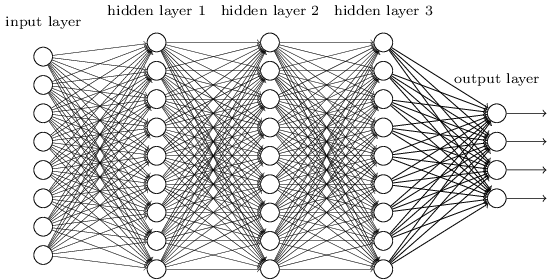
\includegraphics[height=6cm]{img/tikz40.png}
\end{center}

\end{frame}

%%%%%%%%%%%%%%%%%%%%%%%%%%%%%%%%%%%%%%%%%%%%%%%%%%%
\begin{frame}[fragile] \frametitle{} \oldB \small

\yblue{\textbf{Word embeddings}}

A word embedding is nothing more than a compression of a one-hot
representation and a dense hidden layer in a neural network. There
is not need to actually create the one-hot vector, and multiply by
all of $W$. We can just go directly from the index of the word in
the vocabulary, and read off of the $j$-th row of $W$.

\end{frame}

%%%%%%%%%%%%%%%%%%%%%%%%%%%%%%%%%%%%%%%%%%%%%%%%%%%
\begin{frame}[fragile] \frametitle{} \oldB \small

\yblue{\textbf{Word embeddings}}

A word embedding is nothing more than a compression of a one-hot
representation and a dense hidden layer in a neural network. There
is not need to actually create the one-hot vector, and multiply by
all of $W$. We can just go directly from the index of the word in
the vocabulary, and read off of the $j$-th row of $W$.

What are we doing here, really? The whole idea is to map a word as
a vector in a $p$-dimensional space. Much like the bottleneck layer
in an autoencoder, the representation in this space often has a
semantic meaning.

\end{frame}

%%%%%%%%%%%%%%%%%%%%%%%%%%%%%%%%%%%%%%%%%%%%%%%%%%%
\begin{frame}[fragile] \frametitle{} \oldB \small

\yblue{\textbf{Multiple words}}

This is great, but most of the time we want to work with
a collection of words (a document) all as one entity. A
simple way to do this is to apply the word embedding to
each term, and the collapse (flatten) these into a single
long vector.

So if we have $T$ terms in a document and a word embedding
with $p$ terms, the output from the embedding layer will be
of size $T \times p$.

To be clear, the embedding step is agnostic to the position
of the word, much like the shared weights in a convolutional
neural network.

\end{frame}


%%%%%%%%%%%%%%%%%%%%%%%%%%%%%%%%%%%%%%%%%%%%%%%%%%%
\begin{frame}[fragile] \frametitle{} \oldB \small

\yblue{\textbf{Fixed width text}}

We will persist in one simplification today: assuming that
each document has the same number of terms. This is done by
truncating at some small number of words (less than what
most of the movie reviews are) and filling in any trailing
space by a special embedding of zeros.

\end{frame}

%%%%%%%%%%%%%%%%%%%%%%%%%%%%%%%%%%%%%%%%%%%%%%%%%%%
\begin{frame}[fragile] \frametitle{} \oldB \small

\magenta{I. Learning word embeddings with IMDB}

\end{frame}


%%%%%%%%%%%%%%%%%%%%%%%%%%%%%%%%%%%%%%%%%%%%%%%%%%%
\begin{frame}[fragile] \frametitle{} \oldB \small

\yblue{\textbf{Convolutions, again}}

It turns out we can think of the output of the word embeddings
as being similar to the multidimensional tensors in image
processing.

For example, consider a word embedding with $p=3$. We can see
this as three parallel 1-dimensional streams of length $T$,
much in the way that a color image is a 2d-dimensional combination
of parallel red, green, and blue channels.

\pause In this context, we can apply 1-D constitutional layers
just as before: shared weights over some small kernel. Now, however,
the kernel has just a single spatial component.

\end{frame}

%%%%%%%%%%%%%%%%%%%%%%%%%%%%%%%%%%%%%%%%%%%%%%%%%%%
\begin{frame}[fragile] \frametitle{} \oldB \small

\magenta{II. Word embedding with 1D Convolutions}

\end{frame}

%%%%%%%%%%%%%%%%%%%%%%%%%%%%%%%%%%%%%%%%%%%%%%%%%%%
\begin{frame}[fragile] \frametitle{} \oldB \small

\magenta{II. Reuters classification}

\end{frame}

%%%%%%%%%%%%%%%%%%%%%%%%%%%%%%%%%%%%%%%%%%%%%%%%%%%
\begin{frame}[fragile] \frametitle{} \oldB \small

\yblue{\textbf{Transfer learning}}

Much like with the lower convolution layers for image classification,
there is a great benefit to being able to use a large corpus to
learn the word embedding step. And again, we can either treat this
embedding as fixed (transfer learning) or just a good starting point
(pre-training).

\end{frame}

%%%%%%%%%%%%%%%%%%%%%%%%%%%%%%%%%%%%%%%%%%%%%%%%%%%
\begin{frame}[fragile] \frametitle{} \oldB \small

\yblue{\textbf{Autoencoders?}}

We saw that we can either use autoencoders or another classification
task to learn the weights in the levels of a convolutional neural
network.

It turns out that for text, transfer learning with another
classification task does not work quite as well. We instead need
something akin to an autoencoder.

\pause \textbf{Does that seem surprising?}

\end{frame}

%%%%%%%%%%%%%%%%%%%%%%%%%%%%%%%%%%%%%%%%%%%%%%%%%%%
\begin{frame}[fragile] \frametitle{} \oldB \small

\yblue{\textbf{How to autoencode}}

Using a direct autoencoder on a single not make a lot of sense; it would
essentially just boil down to predicting the most frequent words as
well as possible in the bottleneck layer. The latent structure only
comes in when we view a sequence of terms.

\end{frame}

%%%%%%%%%%%%%%%%%%%%%%%%%%%%%%%%%%%%%%%%%%%%%%%%%%%
\begin{frame}[fragile] \frametitle{} \oldB \small

\yblue{\textbf{How to autoencode}}

Using a direct autoencoder on  not make a lot of sense; it would
essentially just boil down to predicting the most frequent words as
well as possible in the bottleneck layer.

Instead, we want to use the context of a word to predict other similar
words that tend to co-occur with it. We'll look at a set of popular
approaches to doing this.

\end{frame}

%%%%%%%%%%%%%%%%%%%%%%%%%%%%%%%%%%%%%%%%%%%%%%%%%%%
\begin{frame}[fragile] \frametitle{} \oldB \small

\yblue{\textbf{Words in context}}

A key idea from the landmark paper
\begin{quote}
Mikolov, Tomas, Ilya Sutskever, Kai Chen, Greg S. Corrado, and
Jeff Dean. "Distributed representations of words and phrases
and their compositionality." In Advances in neural information
processing systems, pp. 3111-3119. (2013).
\end{quote}
And the closely related follow-up:
\begin{quote}
Mikolov, Tomas, Kai Chen, Greg Corrado, and Jeffrey Dean.
"Efficient estimation of word representations in vector space."
arXiv preprint arXiv:1301.3781 (2013).
\end{quote}
Is to try to predict a word given its context. Specifically, we
want to use the context of a word to predict other similar
words that tend to co-occur with it.

\end{frame}

%%%%%%%%%%%%%%%%%%%%%%%%%%%%%%%%%%%%%%%%%%%%%%%%%%%
\begin{frame}[fragile] \frametitle{} \oldB \small

\begin{center}
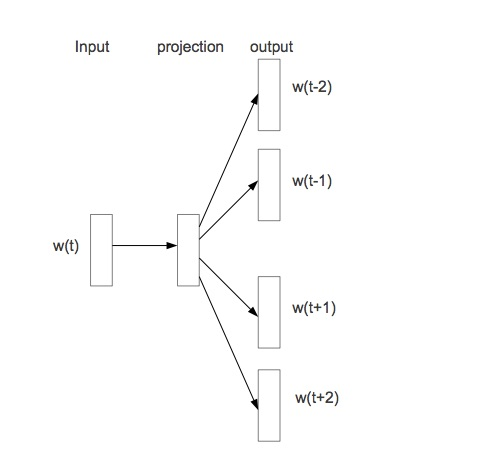
\includegraphics[height=6cm]{img/skipGram.jpg}
\end{center}

\end{frame}

%%%%%%%%%%%%%%%%%%%%%%%%%%%%%%%%%%%%%%%%%%%%%%%%%%%
\begin{frame}[fragile] \frametitle{} \oldB \small

\begin{center}
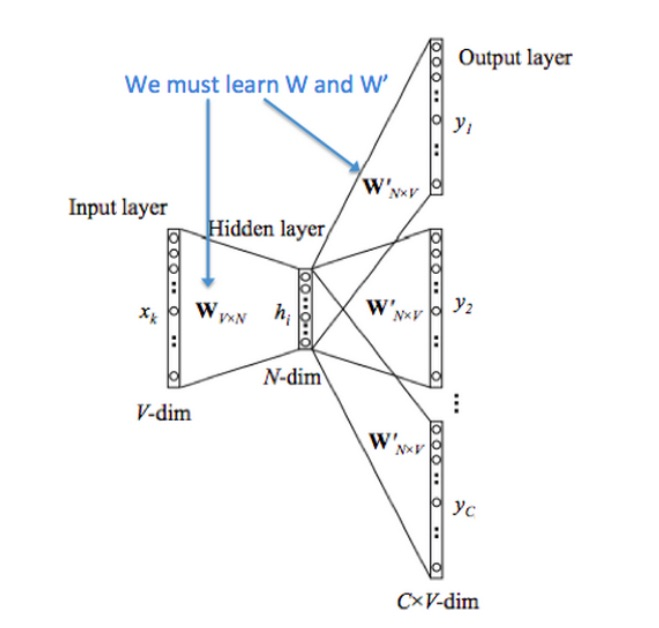
\includegraphics[height=6cm]{img/skipGram2.jpg}
\end{center}

\end{frame}


%%%%%%%%%%%%%%%%%%%%%%%%%%%%%%%%%%%%%%%%%%%%%%%%%%%
\begin{frame}[fragile] \frametitle{} \oldB \small

\begin{center}
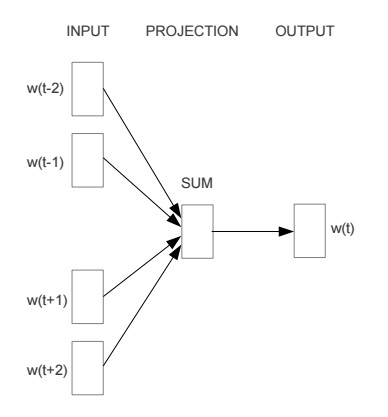
\includegraphics[height=6cm]{img/continuousBagOfWords.jpg}
\end{center}

\end{frame}

%%%%%%%%%%%%%%%%%%%%%%%%%%%%%%%%%%%%%%%%%%%%%%%%%%%
\begin{frame}[fragile] \frametitle{} \oldB \small

\begin{center}
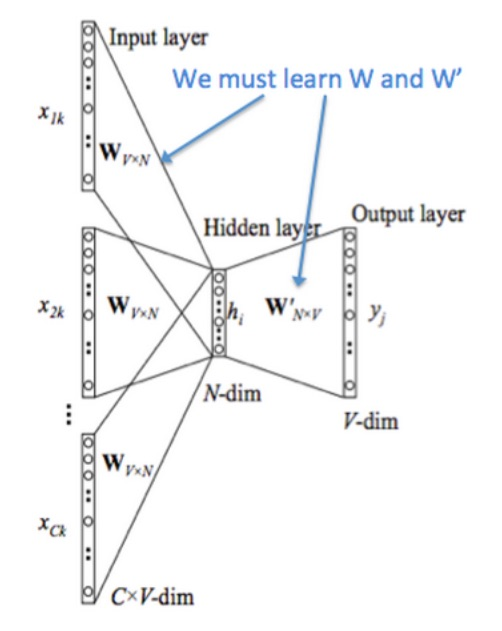
\includegraphics[height=6cm]{img/continuousBagOfWords2.jpg}
\end{center}

\end{frame}


%%%%%%%%%%%%%%%%%%%%%%%%%%%%%%%%%%%%%%%%%%%%%%%%%%%
\begin{frame}[fragile] \frametitle{} \oldB \small

You'll notice that these all yield two representations of
word embeddings. Typically, they are averaged to get the
final set of embeddings to use.

\end{frame}

%%%%%%%%%%%%%%%%%%%%%%%%%%%%%%%%%%%%%%%%%%%%%%%%%%%
\begin{frame}[fragile] \frametitle{} \oldB \small

While we have generally steered away from the more theoretical
papers, I want to draw your attention to one very interesting
one that puts a surprisingly neat theory around word embeddings:
\begin{quote}
Levy, Omer, and Yoav Goldberg. "Neural word embedding as
implicit matrix factorization." In Advances in Neural
Information Processing Systems, pp. 2177-2185. 2014.
\end{quote}
They show that word embeddings essentially amount to a low-rank
factorization of a co-occurrence matrix.

\end{frame}

%%%%%%%%%%%%%%%%%%%%%%%%%%%%%%%%%%%%%%%%%%%%%%%%%%%
\begin{frame}[fragile] \frametitle{} \oldB \small

The specific implementation of these ideas by the Mikolov-headed
group is known as word2vec. They supply pre-coded version of this.
Let's load an example into python:

\magenta{IV. word2vec}

\end{frame}

%%%%%%%%%%%%%%%%%%%%%%%%%%%%%%%%%%%%%%%%%%%%%%%%%%%
\begin{frame}[fragile] \frametitle{} \oldB \small

Another, very closely related technique to word2vec is given
by GloVe:
\begin{quote}
Pennington, Jeffrey, Richard Socher, and Christopher D. Manning.
"GloVe: Global Vectors for Word Representation."
In EMNLP, vol. 14, pp. 1532-1543. (2014).
\end{quote}
The differences are subtle at the level we are talking about,
but you may see references to this model as well in some of the
cited papers.

\end{frame}

%%%%%%%%%%%%%%%%%%%%%%%%%%%%%%%%%%%%%%%%%%%%%%%%%%%
\begin{frame}[fragile] \frametitle{} \oldB \small

Finally, there is still some open questions in the world of
word embeddings. For example, the ideas started with this
paper:
\begin{quote}
Huang, Eric H., Richard Socher, Christopher D. Manning, and
Andrew Y. Ng. "Improving word representations via global
context and multiple word prototypes." In Proceedings of the
50th Annual Meeting of the Association for
Computational Linguistics: Long Papers-Volume 1, pp. 873-882.
Association for Computational Linguistics, 2012.
\end{quote}
Of what to do with the fact that words often have multiple
meanings.

\end{frame}

%%%%%%%%%%%%%%%%%%%%%%%%%%%%%%%%%%%%%%%%%%%%%%%%%%%
\begin{frame}[fragile] \frametitle{} \oldB \small

Finally, there is still some open questions in the world of
word embeddings. For example, the ideas started with this
paper:
\begin{quote}
Huang, Eric H., Richard Socher, Christopher D. Manning, and
Andrew Y. Ng. "Improving word representations via global
context and multiple word prototypes." In Proceedings of the
50th Annual Meeting of the Association for
Computational Linguistics: Long Papers-Volume 1, pp. 873-882.
Association for Computational Linguistics, 2012.
\end{quote}
Of what to do with the fact that words often have multiple
meanings.

\end{frame}

%%%%%%%%%%%%%%%%%%%%%%%%%%%%%%%%%%%%%%%%%%%%%%%%%%%
\begin{frame}[fragile] \frametitle{} \oldB \small

\begin{center}
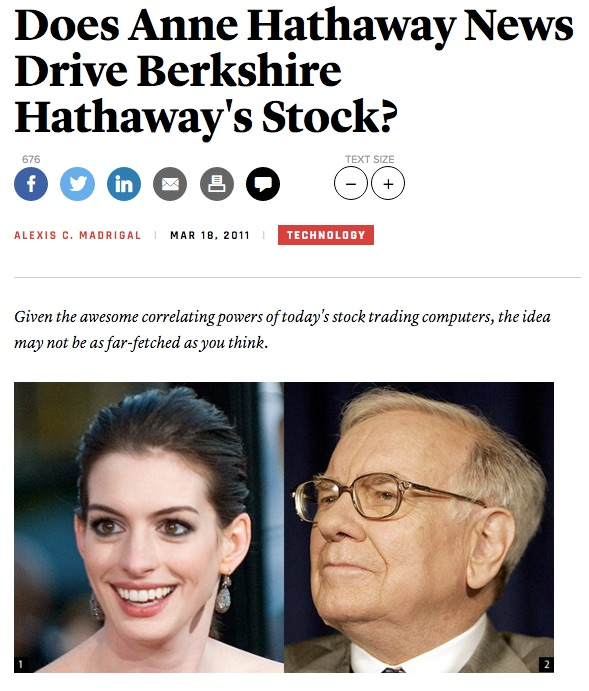
\includegraphics[height=8cm]{img/hathaway.jpg}
\end{center}

\end{frame}




\end{document}







